\documentclass[11pt,letterpaper]{article}
\usepackage{graphicx, geometry, amsmath, amssymb, hyperref, url, natbib, booktabs, xcolor, listings}
\geometry{margin=1in}
\hypersetup{colorlinks=true, linkcolor=black, citecolor=black, urlcolor=black}

\title{Cross-Family Solver Consensus as a Gold-Free Faithfulness Metric\\for Natural-Language-to-First-Order-Logic Translation}

\author{Anonymous}
\date{}

\begin{document}
\maketitle

\begin{abstract}
Evaluating the faithfulness of natural-language-to-first-order-logic (NL$\to$FOL) translations is hampered by the expense and unreliability of gold-standard references: recent audits find that roughly 40\% of annotations in standard benchmarks contain errors.
We study a gold-free alternative based on cross-family solver consensus: collect translations of the same sentence from multiple independent LLM families, check pairwise equivalence with an SMT solver, and score each candidate by the fraction of cross-family peers that disagree with it.
When translators share a supplied predicate vocabulary, consensus achieves a within-template AUROC of 0.954 on 221~fresh long-exception sentences with trusted references and pure Z3 labels, versus 0.587 for a disguised API judge ($\Delta = +0.367$), flat across word-length terciles.
Under free (independently chosen) vocabulary, consensus still outperforms judges on both development data ($\Delta = +0.099$) and untouched out-of-sample sentences ($\Delta = +0.171$, original-view judge), but the advantage shrinks by roughly 0.15~AUROC and a fundamental rename tradeoff emerges: any predicate-name alignment needed to compare independently generated formulas produces a high false-alarm rate on meaning-preserving renames.
Confirmation on independent held-out data was budget-stopped and remains incomplete.
We present these results, identify the conditions under which shared versus free vocabulary governs metric strength, and release the full evaluation code.
\end{abstract}

\section{Introduction}

Translating natural-language sentences into first-order logic (NL$\to$FOL) is a core task in computational semantics and formal verification~\citep{Yang2023,Han2022}.
A correct translation must faithfully capture the meaning of the source sentence: its quantifier scope, polarity, argument structure, and exception clauses.
Evaluating faithfulness is difficult because the same sentence admits many logically equivalent formalizations that differ in predicate names, variable bindings, and structural layout.

Gold-standard references are the default evaluation method, but they are expensive and often wrong.
\citet{Brunello2026} audit two standard benchmarks and find 39--42\% of their annotations contain errors.
This unreliability is not just noise: when the gold reference itself is unfaithful, every metric calibrated against it is miscalibrated.

An alternative is to have a strong LLM judge each translation~\citep{Chiang2024}.
However, LLM judges share failure modes with the translators they evaluate: both are autoregressive models operating on the same distributional statistics, so systematic blind spots tend to be correlated.
As we show in Section~\ref{sec:sig_results}, a cheap disguised judge achieves only 0.587 AUROC on the same sentences where consensus reaches 0.954.

We study a gold-free metric based on cross-family solver consensus.
The idea is simple: if a candidate translation is correct, translations produced independently by other LLM families should be logically equivalent to it.
If the candidate is wrong, independent translators are unlikely to make the same mistake, so their translations will diverge.
We formalise this intuition and evaluate it under two vocabulary regimes:
\begin{enumerate}
\item \textbf{Shared signature}: all translators use a supplied predicate vocabulary. Equivalence checking requires no alignment and labels come from Z3 alone.
\item \textbf{Free vocabulary}: each translator chooses its own predicate names. Equivalence checking requires a predicate-name aligner, which introduces a rename tradeoff (Section~\ref{sec:rename}).
\end{enumerate}

Our contributions:
\begin{itemize}
\item A pre-registered evaluation on 221 long-exception sentences under shared signature: consensus AUROC 0.954 versus 0.587 for the disguised judge ($\Delta = +0.367$ [+0.328, +0.404]), flat across word-length terciles, and 0.956 versus 0.932 for a frontier judge on a descriptive 60-row subsample (Section~\ref{sec:sig_results}). This dataset later served as development data for aligner tuning; the templates and supplied signature limit its scope.
\item Free-vocabulary evaluation on development set~$E$: consensus outperforms judges by $\Delta = +0.099$ [+0.049, +0.146] on stratified AUROC, with aligner-free consensus (c\_exact) at 0.689 [0.652, 0.726] (Section~\ref{sec:dev_results}).
\item Untouched free-vocabulary out-of-sample results on R\_COMP FREE under provisional labels: $\Delta = +0.171$ [+0.135, +0.206] versus the original-view judge; $\Delta = +0.105$ [+0.011, +0.215] on a two-auditor subset; consensus reaches 0.94 of the frontier judge's AUROC (Section~\ref{sec:free_oos}).
\item Documentation of the rename tradeoff: a 76.5\% false-alarm rate under nonce predicate renames that no variant we tested could eliminate without sacrificing error recall (Section~\ref{sec:rename}).
\end{itemize}

\begin{figure}[!htbp]
  \centering
  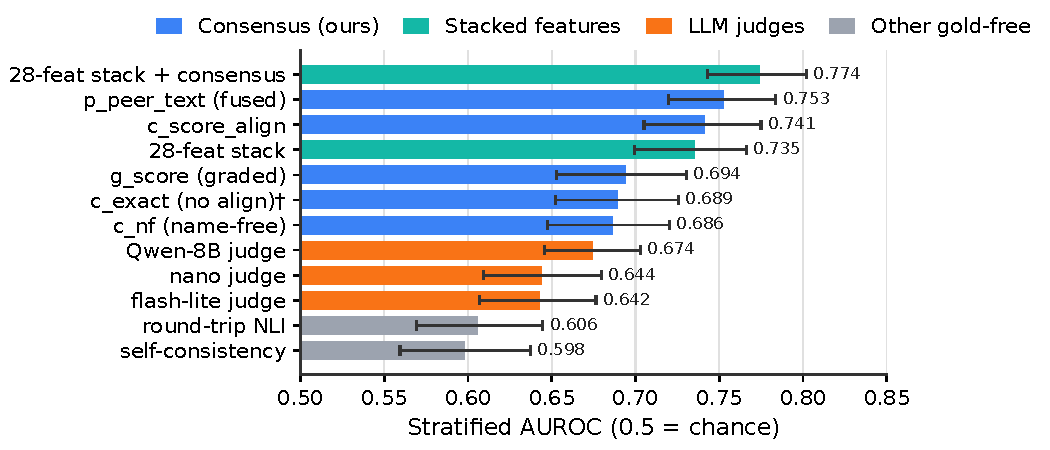
\includegraphics[width=\linewidth,height=0.85\textheight,keepaspectratio]{figures/fig_dev_auroc_v0.pdf}
  \caption{Stratified AUROC on the free-vocabulary development dataset for the main metrics and baselines. Error bars are 95\% sentence-cluster bootstrap confidence intervals. Consensus-based metrics (blue) outperform API judges (orange) and other gold-free baselines (gray).}
  \label{fig:dev_auroc}
\end{figure}

\section{Related Work}

\paragraph{NL\texorpdfstring{$\to$}{-to-}FOL evaluation.}
Standard benchmarks such as FOLIO~\citep{Han2022} and the MALLS corpus~\citep{Yang2023} provide NL--FOL pairs, but gold-annotation error rates are high~\citep{Brunello2026}.
\citet{Vossel2025} map predicates by normalised Levenshtein distance before equivalence checking.
\citet{Thatikonda2025} evaluate n-gram, graph, embedding, and LLM-based closeness metrics on controlled FOL perturbations, finding that no single metric is sensitive to all perturbation types.

\paragraph{Cross-model consensus.}
The idea of using agreement among multiple independently trained models as a quality signal appears in several domains.
\citet{Wang2022} show that sampling multiple chain-of-thought reasoning paths~\citep{Wei2022} from a single model and taking the majority answer (self-consistency) improves accuracy.
\citet{Bayless2025} collect $k$ translations over a fixed shared schema and score each by the fraction of $k$ translations that entail it.
\citet{Zhang2023} detect hallucinations in black-box LLMs by sampling diverse perturbations of a query and checking consistency across answers.
Our work differs from these in evaluating the consensus score under both shared and free vocabulary, head-to-head with API judges, with pre-registered analyses.

\paragraph{LLM-as-judge.}
\citet{Chiang2024} propose using LLMs as evaluators.
In NL$\to$FOL, an LLM judge reads the sentence and the candidate formula and predicts faithfulness.
The disguised variant (nonce predicate names) controls for memorisation of known benchmarks.

\paragraph{Diverse redundancy.}
N-version programming, where independent implementations of the same specification are compared by majority vote, was proposed for software fault tolerance.
\citet{Eckhardt1985} predict that coincident failures rise with input difficulty; our finding that the consensus advantage is flat with sentence length under shared vocabulary but degrades under free vocabulary is consistent with vocabulary alignment, not input difficulty, as the bottleneck.

\section{Method}\label{sec:method}

\subsection{Consensus scoring}

Given a sentence $s$ and a candidate FOL translation $c$, we collect peer translations $\{p_1, \ldots, p_k\}$ from $k$ independent LLM families.\footnote{Code: \url{https://github.com/ai-inventor-papers/ai-invention-eff060-layered-gold-free-checks-for-logic/tree/fork/run_cNhUBrixEdz7/round-1/experiment-1}}
Each peer uses the same few-shot prompt but a different base model (e.g., one from each of Gemini, Claude, GPT, Llama, Qwen, Phi, Mistral).
We compute:
\begin{equation}
\text{c\_score}(c, s) = 1 - \frac{1}{k} \sum_{i=1}^{k} \mathbf{1}[\text{equiv}(c, p_i)]
\end{equation}
where $\text{equiv}(c, p_i)$ checks logical equivalence between $c$ and $p_i$ using the Z3 SMT solver~\citep{Moura2008}.

Under \textbf{shared signature} (c\_score\_sig), all translators use a supplied predicate vocabulary, and equiv is a direct Z3 check after case-insensitive symbol normalisation.
Under \textbf{free vocabulary} (c\_score\_align), each translator chooses its own predicate names, and equiv requires a predicate-name aligner before the Z3 check.

\subsection{Predicate alignment (free vocabulary only)}

Independent translators choose different predicate names for the same concept (e.g., \texttt{Runs(x)} vs.\ \texttt{IsRunner(x)}).
To compare formulas across families, we align predicates using a cost function that combines:
\begin{enumerate}
\item \textbf{Structural cost}: polarity profile, argument-count match, and nesting depth.
\item \textbf{Text-anchor cost}: overlap between predicate-name words and source-sentence tokens (Porter stemming, WordNet synonyms/derivations).
\item \textbf{Semantic signature}: truth-value profiles over random finite interpretations.
\end{enumerate}
The $k$ cheapest bijections (predicates within equal arity; constants separately) are evaluated, and the pair is declared equivalent if any bijection yields a Z3-verified equivalence.

\subsection{Score variants}

Higher scores indicate greater divergence from peers and thus higher predicted error probability.
Variants include:
\begin{itemize}
\item \textbf{c\_exact}: no alignment; exact-match equivalence only. Immune to rename false alarms but blind to vocabulary-differing equivalences.
\item \textbf{c\_nf} (name-free): alignment by structural and semantic signatures only, ignoring text anchoring.
\item \textbf{p\_peer\_text}: a logistic fusion of consensus features with text-side features (bag-of-words coverage, role accounting, Z3 structural match).\footnote{Code: \url{https://github.com/ai-inventor-papers/ai-invention-eff060-layered-gold-free-checks-for-logic/tree/fork/run_cNhUBrixEdz7/round-2/experiment-5}}
\end{itemize}

\subsection{Evaluation framework}

\paragraph{Shared-signature labels.}
On R\_COMP, labels are determined by Z3 equivalence to trusted-by-construction references (one weak and one strong reading per template), with no human or LLM judgement in the labelling loop.

\paragraph{Free-vocabulary labels.}
On development set~$E$, labels come from a three-person expert panel (adjudicated as ERROR or CORRECT), with disputed items counted according to the reliability assignment (R\_AB: both panellists agree).
On R\_COMP FREE, provisional labels use search-based ERROR\_CERT versus MAPPED classifications (non-confirmatory; the gloss-based labelling gate failed twice).

\paragraph{Metrics.}
The primary evaluation metric is stratified AUROC: items are paired only within the same source stratum (sentence-template on R\_COMP, sentence-complexity bin on~$E$), eliminating confounds from stratum-level base rates.
Confidence intervals use sentence-cluster percentile bootstrap ($B = 2{,}000$).

\section{Experiments}\label{sec:experiments}

\subsection{Datasets}

\paragraph{R\_COMP (shared and free vocabulary).}\footnote{Code: \url{https://github.com/ai-inventor-papers/ai-invention-eff060-layered-gold-free-checks-for-logic/tree/fork/run_cNhUBrixEdz7/round-3/experiment-7}}
R\_COMP generates long, complex sentences ($\geq$25 words, 4--5 conditions) from a verified lexicon.
221~sentences produced 2,024 candidate translations from 10~LLM slots across 9~vendor families.
Population: 429~ERROR~/~1,595~CORRECT (21.2\% error rate).
In the \textbf{SIG condition}, all translators received a supplied predicate signature; labels are pure Z3 equivalence to trusted references.
In the \textbf{FREE condition}, each translator chose its own predicate names; labels are provisional (Section~\ref{sec:free_oos}).
The pre-registration document, including the analysis plan and testability rule, was frozen before any SIG generation call, any label, or any metric score.\footnote{Pre-registration: \texttt{prereg\_sig.json}, SHA-256 frozen before data collection.}

\paragraph{Development set $E$.}\footnote{Code: \url{https://github.com/ai-inventor-papers/ai-invention-eff060-layered-gold-free-checks-for-logic/tree/fork/run_cNhUBrixEdz7/round-1/experiment-3}}
8,507~rows from 700~sentences drawn from the MALLS corpus~\citep{Yang2023} and ProverQA~\citep{Qi2025}.
Each sentence was translated by 9~LLM families using a frozen few-shot prompt.
The primary evaluation population (R\_AB, both panellists agree) contains 2,686~items (1,822~ERROR~/~864~CORRECT, 292~sentences); the all-families subset where every peer family contributed a translation is $n = 2{,}014$.
Complexity strata: L25 ($\geq$25 words), L20 (20--24), EXC (exception clauses), CTRL (short control sentences).
The R\_COMP-SIG data later served as development data for aligner tuning, so the development-set numbers from $E$ are not independent of R\_COMP.

\paragraph{Baselines.}
(1)~\textbf{Flash-lite judge} (Gemini Flash Lite, disguised and original views); (2)~\textbf{nano judge} (Gemini Flash 2.0); (3)~\textbf{local judges} (Qwen3-8B, Llama-8B); (4)~\textbf{round-trip NLI}; (5)~\textbf{self-consistency} (5-sample within-model agreement); (6)~\textbf{structural features} (arity consistency, dangling predicates, rerun Jaccard); (7)~\textbf{feature stacks}: cross-validated logistic regressions over subsets of these features.\footnote{Code: \url{https://github.com/ai-inventor-papers/ai-invention-eff060-layered-gold-free-checks-for-logic/tree/fork/run_cNhUBrixEdz7/round-1/experiment-4}}

\subsection{Shared-signature results (R\_COMP-SIG)}\label{sec:sig_results}

Table~\ref{tab:sig} reports the pre-registered comparison on R\_COMP under shared signature.
On the 1,904~rows where both consensus and judge scores exist, consensus achieves a within-template AUROC of 0.954 versus 0.587 for the disguised flash-lite judge ($\Delta = +0.367$ [+0.328, +0.404]).
Against the original-view judge (1,932~rows), the advantage is $\Delta = +0.278$ [+0.239, +0.319].
Error endorsement is zero ($e = 0$): no error item scores below the decision threshold.
Among the 429~error items, 75.3\% receive the maximum consensus score of~1.0; the remaining 24.7\% score between 0.625 and~1.0.

\begin{table}[!htbp]
\centering
\caption{Within-template AUROC on R\_COMP-SIG (shared signature, 221~sentences, pure Z3 labels). CIs are 95\% sentence-cluster bootstrap.}
\label{tab:sig}
\small
\begin{tabular}{lccc}
\toprule
Metric & $n$ & Within-template AUROC [95\% CI] & $\Delta$ vs.\ disg.\ judge [95\% CI] \\
\midrule
c\_score\_sig & 1904 & 0.954 [0.939, 0.968] & +0.367 [+0.328, +0.404] \\
c\_score\_align & 1904 & 0.954 [0.939, 0.968] & +0.367 [+0.328, +0.404] \\
judge (flash-lite, disg.) & 1904 & 0.587 [0.551, 0.622] & --- \\
judge (flash-lite, orig.) & 1932 & 0.673 [0.637, 0.708] & \\
judge (frontier, orig.) & 60 & 0.932 [0.782, 1.000] & \\
judge (local, disg.) & 2024 & 0.498 [0.459, 0.534] & \\
\bottomrule
\end{tabular}
\end{table}

\paragraph{Flat with sentence length.}
Unlike the free-vocabulary setting (Section~\ref{sec:mechanism}), consensus under shared signature is flat across word-length terciles: W1 0.959, W2 0.947, W3 0.953 (Table~\ref{tab:sig_complexity} and Figure~\ref{fig:sig_tercile}).

\begin{table}[!htbp]
\centering
\caption{R\_COMP-SIG within-template AUROC by word-length tercile.}
\label{tab:sig_complexity}
\small
\begin{tabular}{lccccc}
\toprule
Tercile & $n$ & ERR/COR & c\_sig & judge (disg.) & $\Delta$ [CI] \\
\midrule
W1 (shortest) & 574 & 125/449 & 0.959 & 0.578 & +0.382 [+0.278, +0.472] \\
W2 & 743 & 149/594 & 0.947 & 0.624 & +0.331 [+0.253, +0.421] \\
W3 (longest) & 707 & 155/552 & 0.953 & 0.567 & +0.388 [+0.301, +0.471] \\
\bottomrule
\end{tabular}
\end{table}

\begin{figure}[!htbp]
  \centering
  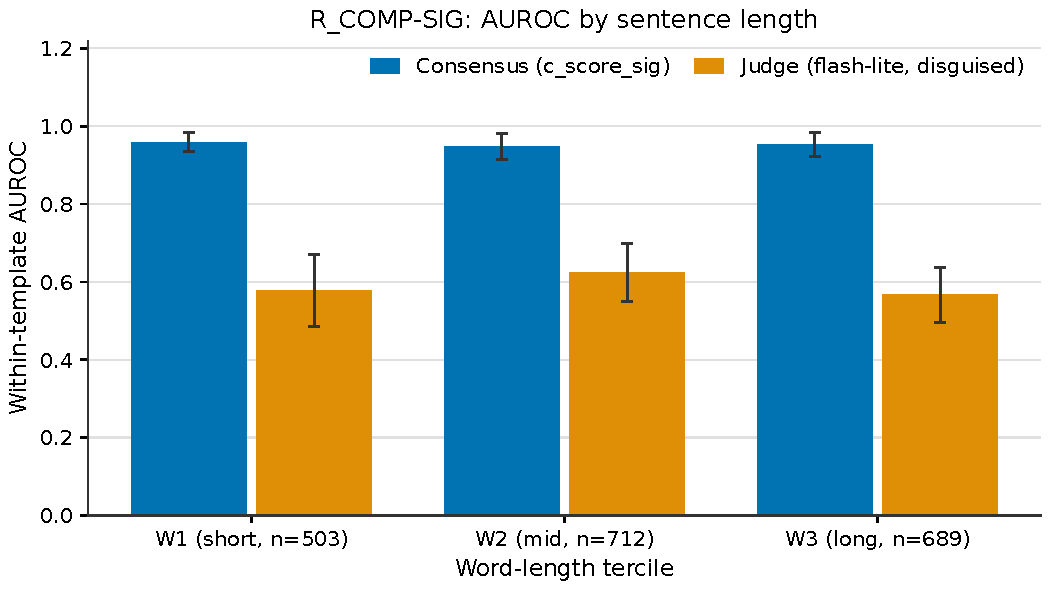
\includegraphics[width=\linewidth,height=0.85\textheight,keepaspectratio]{figures/fig_sig_tercile_v0.pdf}
  \caption{Within-template AUROC on R\_COMP-SIG by word-length tercile. Consensus (blue) is flat across terciles (0.947--0.959), while the disguised flash-lite judge (orange) hovers near chance (0.567--0.624). Error bars are 95\% sentence-cluster bootstrap CIs.}
  \label{fig:sig_tercile}
\end{figure}

\paragraph{Frontier judge comparison.}
On a descriptive 60-row stratified subsample scored by the frontier judge (Gemini~3.1~Pro, original view), consensus achieves pooled AUROC 0.956 [0.889, 1.000] versus 0.932 [0.855, 0.990] for the frontier judge.

\paragraph{Scope.}
R\_COMP-SIG uses templated sentences with a supplied predicate vocabulary.
The shared signature eliminates the alignment problem entirely, which is why the AUROC is so high.
These results do not extend to settings where translators choose their own predicate names.

\subsection{Free-vocabulary development results (set $E$)}\label{sec:dev_results}

Figure~\ref{fig:dev_auroc} and Table~\ref{tab:main} summarise the free-vocabulary comparison on development set~$E$.\footnote{Code: \url{https://github.com/ai-inventor-papers/ai-invention-eff060-layered-gold-free-checks-for-logic/tree/fork/run_cNhUBrixEdz7/round-3/experiment-6}}
Cross-family consensus (c\_score\_align) outperforms the disguised flash-lite judge by $\Delta = +0.099$ [+0.049, +0.146] on the full R\_AB population and by $\Delta = +0.116$ [+0.070, +0.163] on the long-sentence pool (L25+L20+EXC).
Adding c\_score\_align to the 28-feature baseline stack increases stratified AUROC by +0.039 [+0.021, +0.057]; a permutation null test gives $p_{95} = 0.009$, confirming the signal is not explained by the existing features.

\begin{table}[!htbp]
\centering
\caption{Stratified AUROC on development set $E$ (R\_AB population, free vocabulary, $n = 2{,}686$). Higher is better. CIs are 95\% sentence-cluster bootstrap.}
\label{tab:main}
\small
\begin{tabular}{lcc}
\toprule
Metric & Strat AUROC [95\% CI] & \$/item \\
\midrule
c\_score\_align & 0.741 [0.705, 0.775] & 9.1e-5 \\
p\_peer\_text (fused) & 0.753 [0.720, 0.784] & 9.1e-5 \\
c\_exact (no alignment) & 0.689 [0.652, 0.726] & -- \\
c\_nf (name-free) & 0.686 [0.647, 0.720] & -- \\
\midrule
flash-lite judge (disg.) & 0.642 [0.607, 0.676] & 5.1e-5 \\
flash-lite judge (orig.) & 0.623 [0.593, 0.651] & 5.1e-5 \\
nano judge (disg.) & 0.644 [0.609, 0.680] & 2.0e-5 \\
local judge Qwen-8B (disg.) & 0.674 [0.646, 0.703] & -- \\
\midrule
round-trip NLI (min) & 0.606 [0.569, 0.645] & 2.8e-5 \\
self-consistency (5-sample) & 0.598 [0.559, 0.637] & 6.7e-5 \\
\midrule
28-feature stack & 0.735 [0.699, 0.766] & -- \\
28-feature stack + c\_score\_align & 0.774 [0.743, 0.802] & -- \\
\bottomrule
\end{tabular}
\end{table}

The drop from 0.952 (shared signature, R\_COMP-SIG) to 0.801 (free vocabulary on the same R\_COMP sentences) reflects the cost of predicate-name alignment: the aligner introduces both false negatives (correct equivalences missed) and false positives (incorrect mappings endorsed).
Aligner-free consensus (c\_exact) achieves 0.689 [0.652, 0.726]; the aligner adds about 22\% of the above-chance signal (c\_align 0.241 versus c\_exact 0.189 above the 0.5 baseline), with the remaining 78\% coming from structural agreement alone.

On L25 sentences alone ($\geq$25 words), the advantage narrows to $\Delta = +0.069$ [$-$0.020, +0.148], not significant at the 95\% level.
This foreshadows the length-dependent degradation described in Section~\ref{sec:mechanism}.

\paragraph{Frontier judge comparison.}
On the 284-row subsample scored by the frontier judge (Gemini~3.1~Pro), c\_score\_align achieves 95.7\% of the frontier judge's AUROC (ratio 0.957 [0.887, 1.034]).

\paragraph{System-level ranking.}
The consensus metric achieves Kendall $\tau_b = 0.692$ [+0.513, +0.795] between system mean score and R\_AB error rate across 13 system$\times$variant configurations, comparable to the best judges.

\subsection{Free-vocabulary out-of-sample (R\_COMP FREE)}\label{sec:free_oos}

The same 221~R\_COMP sentences were also translated under free vocabulary (each translator choosing its own predicate names).\footnote{Code: \url{https://github.com/ai-inventor-papers/ai-invention-eff060-layered-gold-free-checks-for-logic/tree/fork/run_cNhUBrixEdz7/round-5/experiment-13}}
Confirmatory labelling required a gloss gate (LLM-checked semantic alignment of predicate mappings).
This gate failed twice (balanced accuracy 0.776 and 0.561, below the 0.90 threshold), producing zero confirmed CORRECT rows and rendering the confirmatory test not testable.

Under provisional non-confirmatory labels (ERROR\_CERT vs.\ MAPPED, where MAPPED is an upper bound on CORRECT), Table~\ref{tab:free} reports the untouched results.

\begin{table}[!htbp]
\centering
\caption{R\_COMP FREE provisional AUROCs (within-template, untouched rows). Labels are non-confirmatory.}
\label{tab:free}
\small
\begin{tabular}{lccc}
\toprule
View & $n$ (ERR/MAPPED) & c\_align & judge \\
\midrule
Disguised & 1706 (602/1104) & 0.801 [0.770, 0.834] & 0.584 [0.550, 0.618] \\
Original & 1709 (605/1104) & 0.804 [0.774, 0.836] & 0.633 [0.601, 0.666] \\
\bottomrule
\end{tabular}
\end{table}

The disguised-judge delta is $+0.217$ [+0.175, +0.260]; the original-view delta is $+0.171$ [+0.135, +0.206].
On a 146-row subset with independent two-auditor labels, consensus achieves $\Delta = +0.105$ [+0.011, +0.215] over the original-view judge.
On a 150-row frontier-judge subsample, consensus reaches 0.94 of the frontier judge's AUROC (ratio 0.940 [0.825, 1.056]).

These provisional numbers cannot count as confirmation because the MAPPED labels conflate vocabulary-alignment failures with genuine correctness.
They are consistent with the development-set signal but independent confirmation requires a working gloss gate or a different labelling strategy.

\subsection{Mechanism}\label{sec:mechanism}

We decompose the consensus signal\footnote{Code: \url{https://github.com/ai-inventor-papers/ai-invention-eff060-layered-gold-free-checks-for-logic/tree/fork/run_cNhUBrixEdz7/round-3/evaluation-2}} into two components at a fixed decision threshold:
\begin{itemize}
\item \textbf{Endorsement} $e$: fraction of ERROR items endorsed by the peer majority (false negatives of consensus).
\item \textbf{Divergence} $d$: fraction of CORRECT items that diverge from the peer majority (false positives of consensus).
\end{itemize}
The consensus AUROC at a binary threshold equals $1 - (e + d)/2$, so both quantities must be small for the metric to work.

\paragraph{Shared vocabulary: endorsement zero, divergence moderate.}
On R\_COMP-SIG, $e = 0.0$ and $d = 0.260$: no error escapes detection, though 26\% of correct translations are flagged as divergent.
The false-alarm rate of 0.260 arises from correct translations that use valid but structurally different formalizations; because all translators share a predicate vocabulary, no alignment step is needed and the divergence rate is flat across sentence lengths.

\paragraph{Free vocabulary: divergence degrades with length.}
As Figure~\ref{fig:complexity} shows, on development set~$E$ the net consensus degradation from short to long sentences is $\Delta(e+d) = +0.356$ [+0.198, +0.493], driven almost entirely by divergence ($\Delta d = +0.608$, $\Delta e = -0.252$): as formulas grow longer and more structurally diverse, the predicate-name aligner (Section~\ref{sec:rename}) increasingly maps distinct predicates together or fails to match equivalent ones, inflating the false-alarm rate on correct translations.

\begin{figure}[!htbp]
  \centering
  
\includegraphics[width=\linewidth,height=0.85\textheight,keepaspectratio]{figures/fig_complexity_v0.pdf}
  \caption{Decomposition of free-vocabulary consensus error rates by sentence-length tercile on development set~$E$. Endorsement rate $e$ (errors incorrectly endorsed by peers) decreases with length, but divergence rate $d$ (correct items incorrectly flagged) increases sharply, producing net degradation of +0.356 from the shortest to the longest tercile. Under shared signature (R\_COMP-SIG), this degradation is absent.}
  \label{fig:complexity}
\end{figure}

\paragraph{Family sufficiency.}
Three peer families suffice for 97\% of full-pool AUROC ($k_{95} = 3$), but the long-sentence tercile requires $k_{95} = 5$ (Table~\ref{tab:k_families} and Figure~\ref{fig:k_curve}).

\begin{table}[!htbp]
\centering
\caption{Free-vocabulary AUROC by number of peer families on development set $E$.}
\label{tab:k_families}
\small
\begin{tabular}{ccc}
\toprule
$k$ & AUROC (overall) & AUROC (long, T3) \\
\midrule
1 & 0.685 & 0.581 \\
3 & 0.757 & 0.651 \\
5 & 0.776 & 0.698 \\
7 & 0.784 & 0.726 \\
\bottomrule
\end{tabular}
\end{table}

\begin{figure}[!htbp]
  \centering
  
\includegraphics[width=\linewidth,height=0.85\textheight,keepaspectratio]{figures/fig_k_curve_v0.pdf}
  \caption{Stratified AUROC as a function of the number of peer families $k$, for the full development set (solid blue) and the long-sentence tercile (dashed red). Three families capture 97\% of the full-pool signal, but long sentences require five families to reach 95\%.}
  \label{fig:k_curve}
\end{figure}

\subsection{Confirmation status}\label{sec:confirmation}

Independent confirmation on held-out data remains incomplete.
A fresh held-out dataset (E2-A, 550~new sentences) was constructed, but the run-level budget was exhausted before enough items could be labelled.\footnote{Code: \url{https://github.com/ai-inventor-papers/ai-invention-eff060-layered-gold-free-checks-for-logic/tree/fork/run_cNhUBrixEdz7/round-4/dataset-4}}
On the one testable stratum (DT, short sentences from ProverQA), consensus achieves a stratified AUROC of 0.916, tying the local Qwen-8B judge ($\Delta = +0.003$ [$-$0.042, +0.052]).
On L25 sentences, c\_score\_align falls to 0.443 on only 42 items (35~ERROR~/~7~CORRECT), below chance, but the estimate has extreme variance with only 7~CORRECT items from 3~sentences.
Every pre-registered criterion on the target strata returned NOT\_TESTABLE or unfavourable.

\subsection{The rename tradeoff}\label{sec:rename}

The predicate aligner\footnote{Code: \url{https://github.com/ai-inventor-papers/ai-invention-eff060-layered-gold-free-checks-for-logic/tree/fork/run_cNhUBrixEdz7/round-3/experiment-8}} that enables cross-family comparison under free vocabulary also introduces a fundamental false-alarm vulnerability.
When correct formulas are copied with meaning-preserving predicate renames (same semantics, different symbol names), the consensus score should not change.
Table~\ref{tab:rename} shows the false-alarm rates in practice.

\begin{table}[!htbp]
\centering
\caption{False-alarm (FA) rates on meaning-preserving renames of CORRECT candidates. NONCE = random nonsense names; SYN = WordNet synonyms. Flip = FA induced by the rename alone (FA minus base FA).}
\label{tab:rename}
\small
\begin{tabular}{lcccc}
\toprule
Metric & NONCE FA & NONCE flip & SYN FA & SYN flip \\
\midrule
c\_align & 0.765 & 0.605 & 0.565 & 0.313 \\
c\_nf (name-free) & 0.132 & 0.000 & 0.201 & 0.000 \\
p\_peer\_text & 1.000 & 0.821 & 0.216 & 0.080 \\
judge (disg.) & 0.229 & 0.134 & 0.085 & 0.058 \\
\bottomrule
\end{tabular}
\end{table}

The name-free variant c\_nf eliminates rename sensitivity (flip = 0) but at the cost of blindness to meaning-rename errors (within-base AUROC 0.499, chance level) and lower overall discrimination (strat AUROC 0.686 vs.\ 0.741).
This tradeoff explains the gap between shared-signature and free-vocabulary performance: the shared signature eliminates the need for alignment entirely, sidestepping the rename problem.

\subsection{Per-type sensitivity}

On the PERTURB suite (4,234 typed mutants + 868 controls from development data), consensus recall at the primary threshold is flat across error operators: NEG 0.761, SWAP 0.758, DROP 0.721, ADD 0.763, MEANING\_RENAME 0.762.
Per-operator AUROC within error types cannot be computed because 94--100\% of mutants receive the maximum consensus score, a ceiling effect of the endorsement structure.

Error typing outside a shared vocabulary is negative: the free-vocabulary typing accuracy is 0.123 [0.081, 0.169] on $E$, below both the judge (0.326) and the peer-medoid baseline (0.328), and all three are near chance for a five-class task.

\subsection{Dead ends}

Several alternatives were investigated and abandoned during development: a fused structural-feature filter (false-alarm gate failure); name-free consensus c\_nf (rename-invariant but blind to meaning-rename errors, as described in Section~\ref{sec:rename}); a decomposed solver-based semantic reader (balanced accuracy 0.476); LLM adjudication of disputed items (balanced accuracy 0.662 on expert-labelled items); and candidate-signature consensus, which scores candidates by cueing peers with the candidate's own predicate symbols rather than letting them choose independently (provisional negative: error endorsement rose to 0.459 because peers were anchored into reproducing the candidate's errors).\footnote{Code: \url{https://github.com/ai-inventor-papers/ai-invention-eff060-layered-gold-free-checks-for-logic/tree/fork/run_cNhUBrixEdz7/round-4/experiment-9}}

\section{Discussion}

\subsection{Shared versus free vocabulary}

The central finding is that vocabulary regime governs metric strength.
Under shared signature, consensus achieves near-perfect discrimination (0.954 AUROC) flat across sentence lengths.
Under free vocabulary, performance drops by roughly 0.15~AUROC on comparable sentences (R\_COMP-SIG 0.952 versus R\_COMP FREE 0.801, both within-template on long composed sentences) and degrades with sentence length on natural data.

This gap is explained by the rename tradeoff: the predicate-name aligner needed for free-vocabulary comparison introduces both false negatives (missed equivalences) and false positives (spurious mappings), and these grow worse as formulas become longer and more structurally diverse.
The practical implication is that consensus-based evaluation is most reliable when translators share a predicate vocabulary, as in controlled evaluation settings~\citep{Bayless2025,Vossel2025}.

\subsection{Why confirmation is incomplete}

The confirmation attempt was defeated by two independent problems: (1)~insufficient fresh data (the E2-A budget was stopped before enough correct items accumulated in the long-sentence strata), and (2)~a broken labelling gate (the gloss-based semantic alignment required for R\_COMP FREE labels failed quality checks twice).
Neither failure refutes the development-set signal, but neither allows us to confirm it on the target strata.

The E2-A L25 result (AUROC 0.443, near chance, on 42~items) is concerning but difficult to interpret: with only 7~CORRECT items from 3~sentences, the estimate has extreme variance and a single sentence can dominate.
We report it for completeness but note that it does not meet any standard testability criterion.

\subsection{The rename tradeoff as a fundamental limit}

The rename tradeoff is not a bug in our aligner but a structural property of cross-family consensus under independent vocabulary.
Any alignment procedure that maps independently chosen predicate names to a common vocabulary will sometimes map semantically distinct predicates together, endorsing meaning-rename errors.
Eliminating the alignment (c\_exact, c\_nf) preserves rename invariance but sacrifices the structural comparison that drives error detection.

We conjecture that resolving this tradeoff requires either (a)~a shared predicate vocabulary supplied to all translators, which eliminates the problem entirely but restricts the evaluation to controlled settings~\citep{Bayless2025,Vossel2025}, or (b)~a semantic disambiguation step (such as natural-language glosses of each predicate) that could break the alignment ambiguity.
Our attempt at option~(b), a gloss gate using LLM-generated explanations of predicate meanings, failed quality checks, leaving this direction open.

\subsection{Limitations}\label{sec:limitations}

\begin{enumerate}
\item \textbf{Shared-signature scope.} The 0.954 AUROC result uses templated sentences with a supplied predicate vocabulary, which eliminates the alignment problem. The templates and the supplied signature limit the scope of this result to controlled evaluation settings.
\item \textbf{Development data overlap.} The R\_COMP-SIG dataset later served as development data for aligner tuning. The pre-registration ensures the SIG result itself is uncontaminated, but the development-set numbers from $E$ are not independent.
\item \textbf{Rename vulnerability.} Under free vocabulary, a 76.5\% false-alarm rate on nonce renames means the metric will systematically penalise any translation that uses non-standard predicate names, even if semantically correct.
\item \textbf{Length degradation (free vocabulary).} Consensus discrimination degrades with sentence length under free vocabulary (NET $+0.356$), driven by correct-translation divergence. The metric is weakest on the longest, most complex sentences, precisely the cases where gold-free evaluation is most needed.
\item \textbf{Provisional labels.} R\_COMP FREE results use provisional (non-confirmatory) labels; the two-auditor subset ($\Delta = +0.105$) has a CI that barely excludes zero.
\item \textbf{Label dependence.} Development results on~$E$ depend on a three-person panel whose agreement is imperfect (disputed items exist in every stratum). The metric's advantage could partly reflect alignment with panel biases rather than with ground-truth faithfulness.
\item \textbf{Cost.} The consensus metric requires generating $k$ peer translations per sentence. In this experiment ($k = 9$, R\_COMP-SIG), the amortised consensus cost per candidate is about 19 times the cost of a single cheap judge call.
\item \textbf{Domain.} All results are on English$\to$FOL from MALLS, ProverQA, and R\_COMP sources. Generalisation to other logic formalisms, languages, or sentence distributions is untested.
\end{enumerate}

\section{Conclusion}

Cross-family solver consensus is a strong gold-free faithfulness metric for NL$\to$FOL translation when translators share a predicate vocabulary.
The pre-registered R\_COMP-SIG result (AUROC 0.954 versus 0.587 for a disguised judge, flat with length) establishes the ceiling; free vocabulary costs roughly 0.15~AUROC and introduces the rename tradeoff.

Under free vocabulary, consensus still outperforms cheap LLM judges on both development data ($+0.099$) and untouched out-of-sample sentences ($+0.171$), and adds information beyond structural and statistical baselines.
The mechanism --- errors scatter while correct translations cluster --- provides an intuitive explanation grounded in the diversity of independent formalizations.

However, independent confirmation on held-out data was budget-stopped and remains incomplete, the rename tradeoff limits applicability to free-vocabulary settings, and discrimination degrades with sentence length under free vocabulary.
We release the full evaluation code and data to enable reproduction.
The immediate open problems are: (1)~completing the fresh-data confirmation with adequate sample sizes; (2)~breaking the rename tradeoff, perhaps through semantic predicate glossing; and (3)~understanding why correct translations of complex sentences diverge under free vocabulary even when no vocabulary mismatch exists.

\bibliographystyle{plainnat}
\bibliography{references}

\end{document}
